\documentclass{article}
\usepackage[utf8]{inputenc}
\usepackage{booktabs}
\usepackage{graphicx}
\usepackage{float}
\usepackage{siunitx}
\title{Rocket Stage Optimization Results}
\author{Generated by Stage\_Opt}
\date{February 23, 2025}

\begin{document}
\maketitle

\section{Introduction}
This report presents the results of optimizing a multi-stage rocket using various optimization methods. The objective was to mazimize the payload mass fraction while satisfying the total delta-V requirement.

\section{Input Assumptions}
\subsection{Global Parameters}
\begin{table}[H]
\centering
\caption{Global Parameters}
\begin{tabular}{lS[table-format=4.2]}
\toprule
Parameter & {Value} \\
\midrule
Gravitational Acceleration ($G_0$) & \SI{9.81}{\meter\per\second\squared} \\
Total $\Delta V$ Required & \SI{0.0}{\meter\per\second} \\
\bottomrule
\end{tabular}
\end{table}

\subsection{Stage Parameters}
\begin{table}[H]
\centering
\caption{Stage Parameters and Assumptions}
\begin{tabular}{cS[table-format=3.0]S[table-format=1.3]}
\toprule
Stage & {ISP (\si{\second})} & {Mass Fraction ($\epsilon$)} \\
\midrule
1 & 300 & 0.150 \\
2 & 348 & 0.100 \\
3 & 400 & 0.040 \\
\bottomrule
\end{tabular}
\end{table}

\section{Optimization Methods}
The following optimization methods were evaluated:
\begin{itemize}
\item SLSQP
\item BASIN-HOPPING
\item GA
\item ADAPTIVE-GA
\item DE
\item PSO
\end{itemize}

\section{Optimization Results}
\subsection{Performance Visualization}
\begin{figure}[H]
\centering
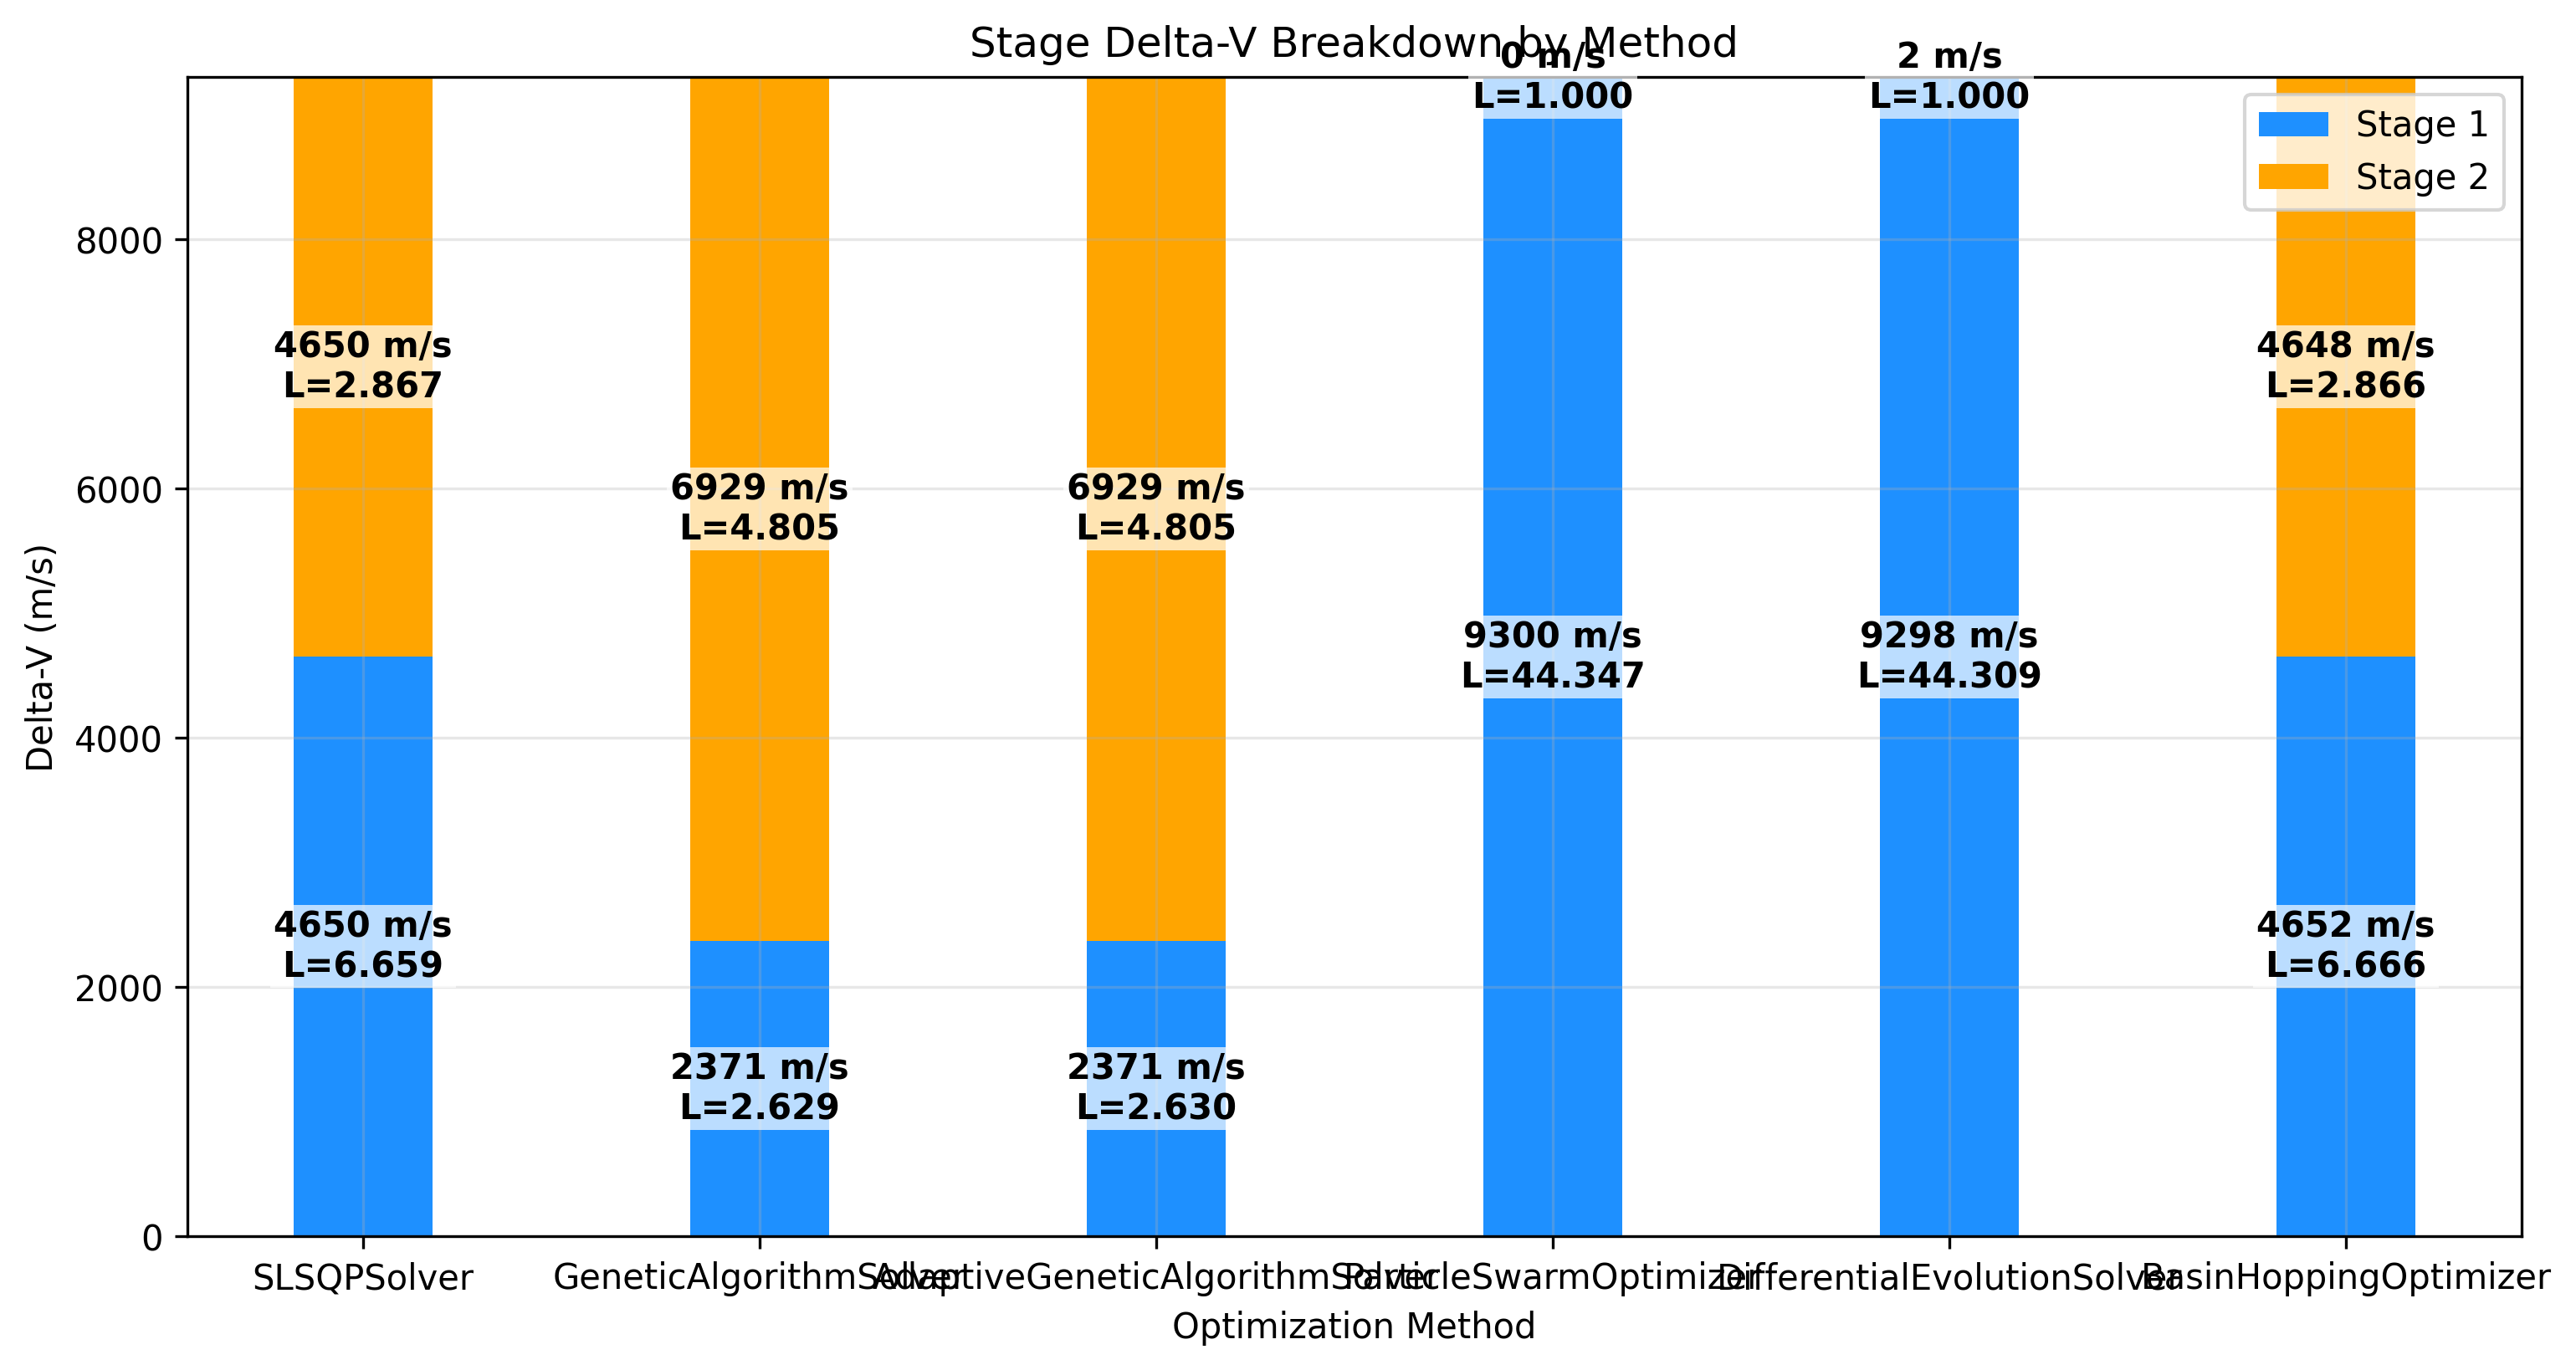
\includegraphics[width=1.2\textwidth]{dv_breakdown.png}
\caption{$\Delta V$ Distribution Across Stages}
\end{figure}

\begin{figure}[H]
\centering
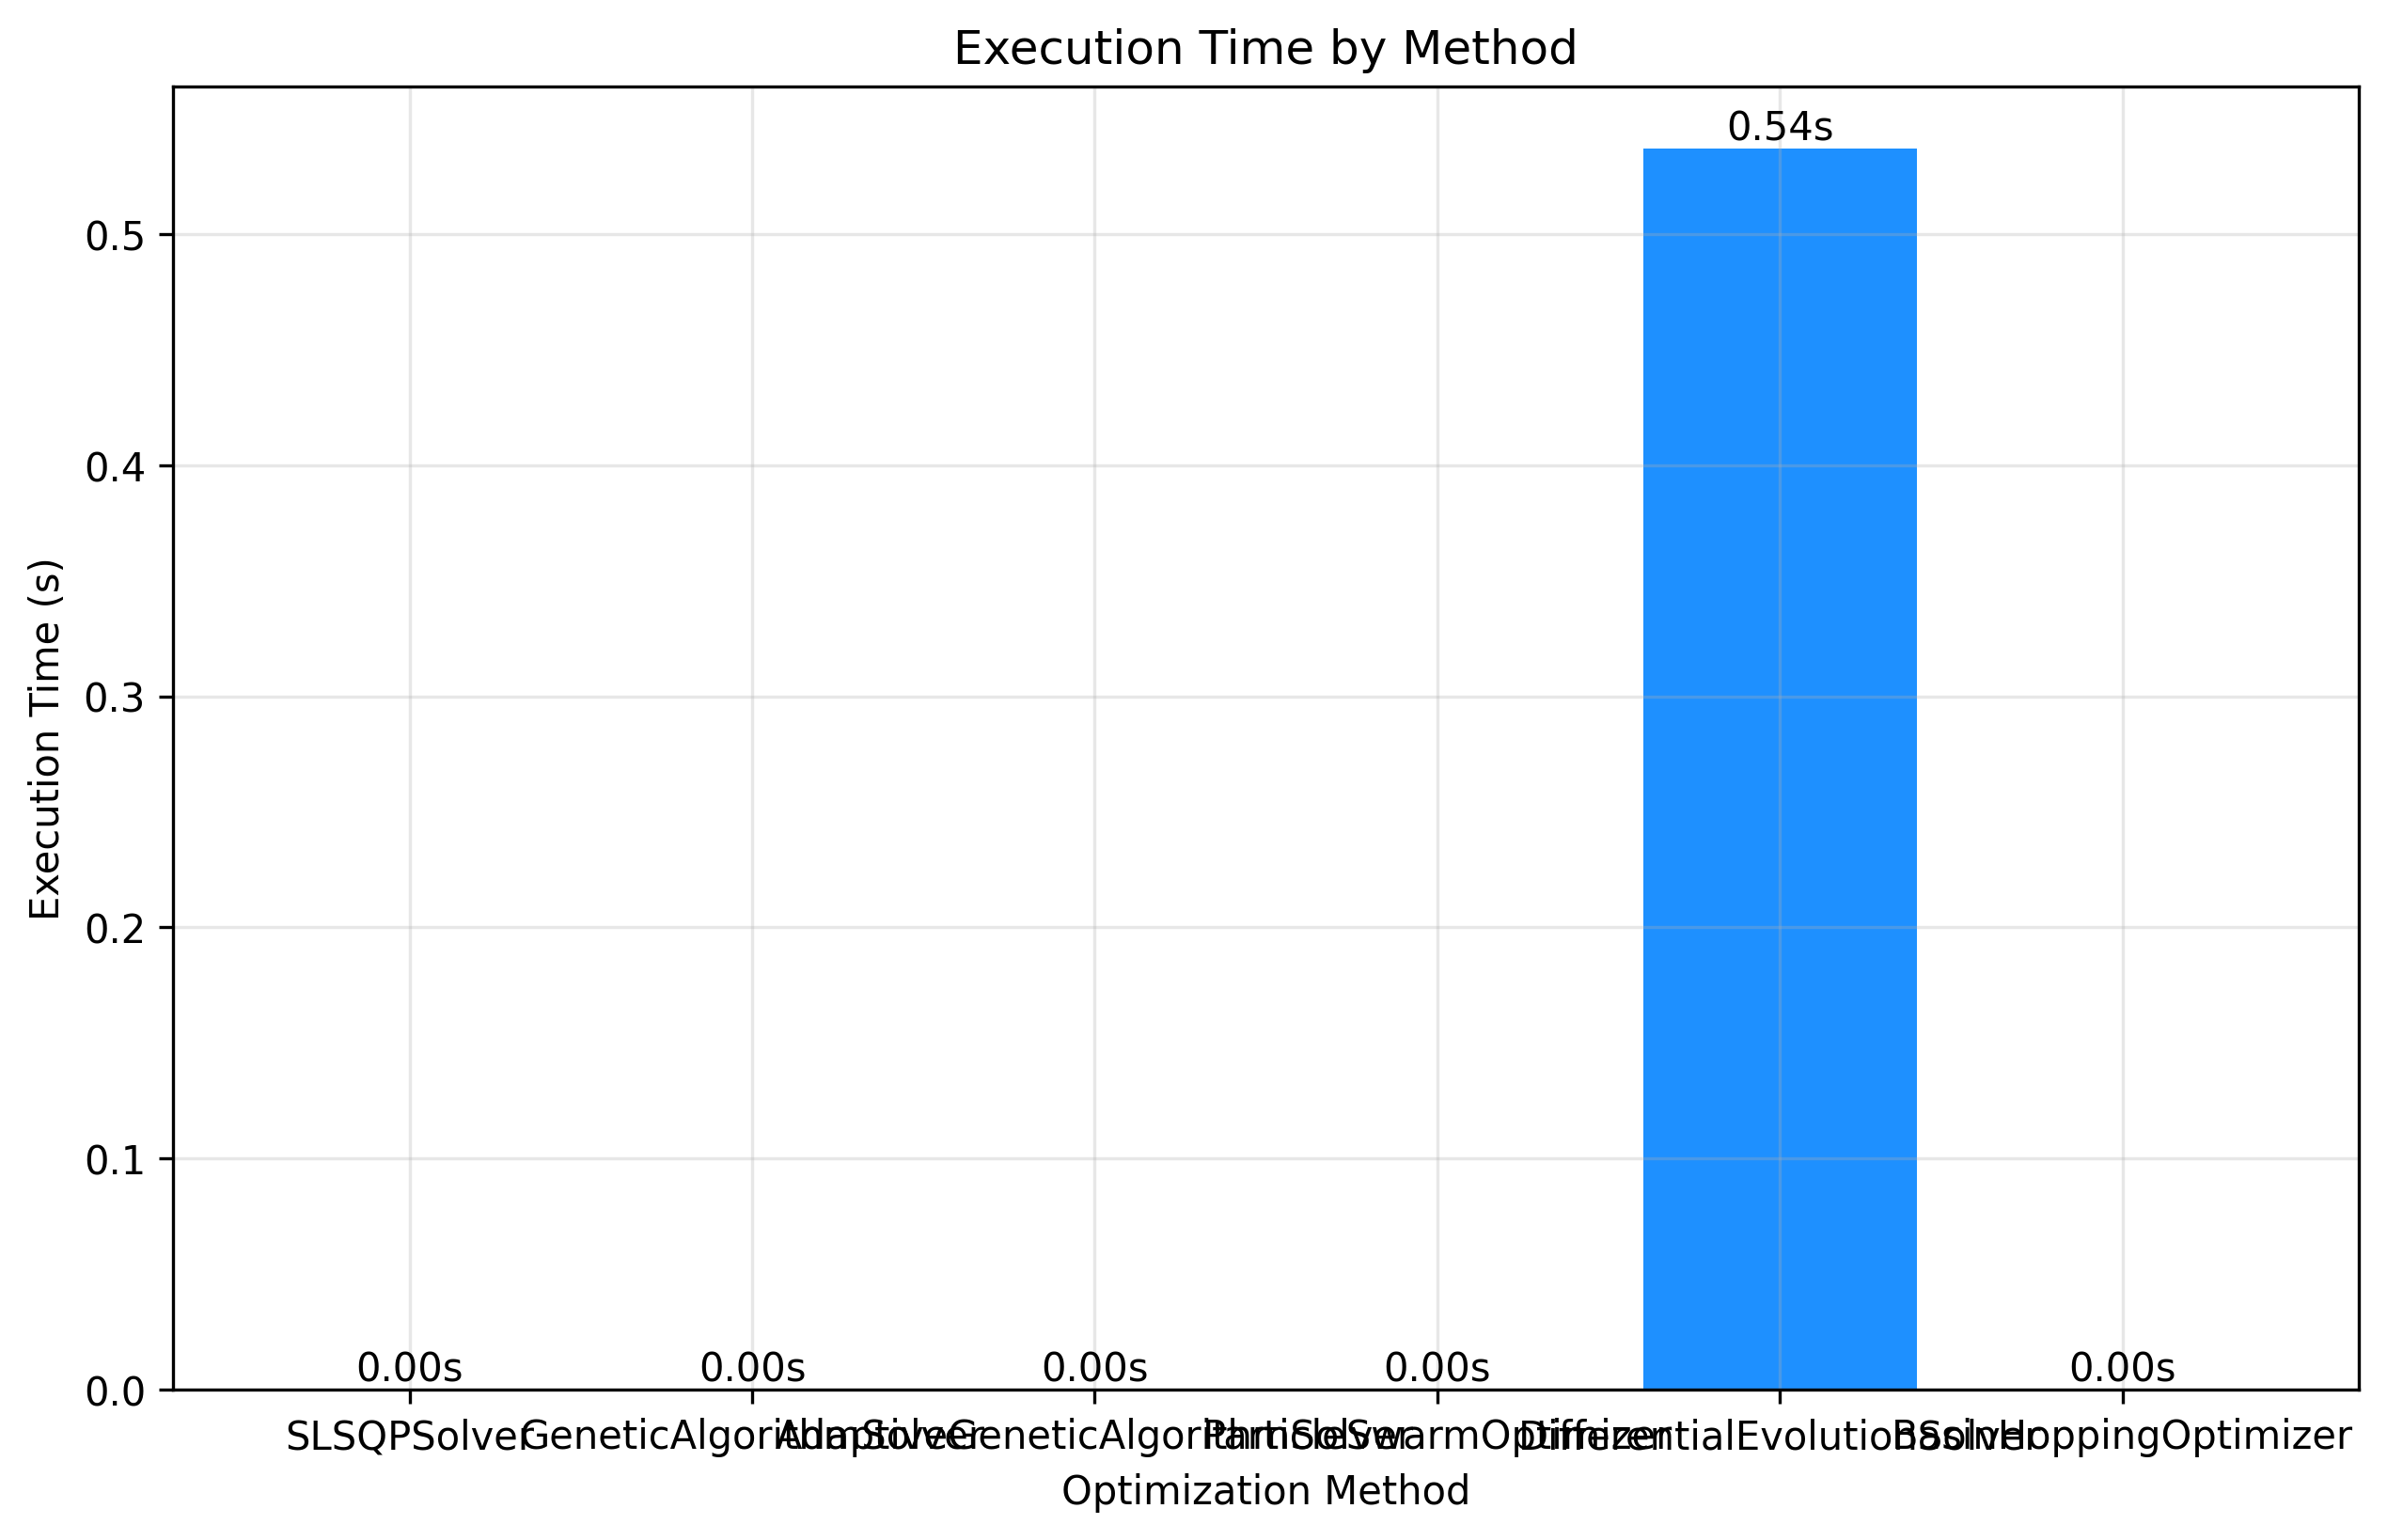
\includegraphics[width=\textwidth]{execution_time.png}
\caption{Solver Execution Time Comparison}
\end{figure}

\begin{figure}[H]
\centering
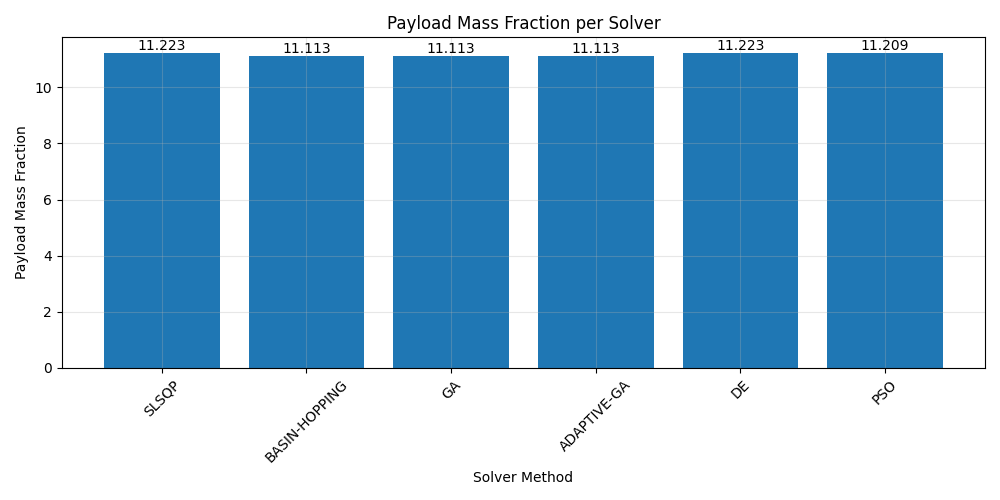
\includegraphics[width=\textwidth]{payload_fraction.png}
\caption{Payload Fraction Comparison}
\end{figure}

\section{Final Results Summary}
\begin{table}[H]
\centering
\caption{Optimization Results Summary}
\begin{tabular}{lS[table-format=1.4]S[table-format=1.4e-1]S[table-format=1.2]}
\toprule
Method & {Payload Fraction} & {Error} & {Time (\si{\second})} \\
\midrule
SLSQP        & 0.0249 & 0.0000e+00 & 0.00 \\
BASIN-HOPPING & 0.0249 & 0.0000e+00 & 1.79 \\
GA           & 0.0249 & 0.0000e+00 & 4.65 \\
ADAPTIVE-GA  & 0.0249 & 0.0000e+00 & 0.05 \\
DE           & 0.0403 & 0.0000e+00 & 1.11 \\
PSO          & 0.0403 & 0.0000e+00 & 0.36 \\
\bottomrule
\end{tabular}
\end{table}

\subsection{Stage-by-Stage Analysis}

% Individual Stage Comparisons

\begin{table}[H]
\centering
\caption{Stage 1 Comparison Across Methods}
\begin{tabular}{lS[table-format=4.1]S[table-format=1.4]S[table-format=3.1]}
\toprule
Method & {$\Delta V$ (\si{\meter\per\second})} & {Mass Ratio ($\lambda$)} & {Contribution (\%)} \\
\midrule
SLSQP        & 3100.0 & 0.1988 & 33.3 \\
BASIN-HOPPING & 3100.3 & 0.1987 & 33.3 \\
GA           & 3100.0 & 0.1988 & 33.3 \\
ADAPTIVE-GA  & 3100.0 & 0.1988 & 33.3 \\
DE           & 1395.0 & 0.4725 & 15.0 \\
PSO          & 1395.0 & 0.4725 & 15.0 \\
\bottomrule
\end{tabular}
\end{table}

\begin{table}[H]
\centering
\caption{Stage 2 Comparison Across Methods}
\begin{tabular}{lS[table-format=4.1]S[table-format=1.4]S[table-format=3.1]}
\toprule
Method & {$\Delta V$ (\si{\meter\per\second})} & {Mass Ratio ($\lambda$)} & {Contribution (\%)} \\
\midrule
SLSQP        & 3100.0 & 0.3033 & 33.3 \\
BASIN-HOPPING & 3100.1 & 0.3033 & 33.3 \\
GA           & 3100.0 & 0.3033 & 33.3 \\
ADAPTIVE-GA  & 3100.0 & 0.3033 & 33.3 \\
DE           & 848.7 & 0.6799 & 9.1 \\
PSO          & 848.8 & 0.6799 & 9.1 \\
\bottomrule
\end{tabular}
\end{table}

\begin{table}[H]
\centering
\caption{Stage 3 Comparison Across Methods}
\begin{tabular}{lS[table-format=4.1]S[table-format=1.4]S[table-format=3.1]}
\toprule
Method & {$\Delta V$ (\si{\meter\per\second})} & {Mass Ratio ($\lambda$)} & {Contribution (\%)} \\
\midrule
SLSQP        & 3100.0 & 0.4138 & 33.3 \\
BASIN-HOPPING & 3099.5 & 0.4139 & 33.3 \\
GA           & 3100.0 & 0.4138 & 33.3 \\
ADAPTIVE-GA  & 3100.0 & 0.4138 & 33.3 \\
DE           & 7056.3 & 0.1256 & 75.9 \\
PSO          & 7056.2 & 0.1256 & 75.9 \\
\bottomrule
\end{tabular}
\end{table}

% Overall Stage Distribution Analysis
\begin{table}[H]
\centering
\caption{Stage Distribution Summary}
\begin{tabular}{lS[table-format=4.1]S[table-format=4.1]S[table-format=4.1]S[table-format=1.4]}
\toprule
Method & {Stage 1 (\%)} & {Stage 2 (\%)} & {Stage 3 (\%)} & {Total $\lambda$} \\
\midrule
SLSQP        & 33.3 & 33.3 & 33.3 & 0.0249 \\
BASIN-HOPPING & 33.3 & 33.3 & 33.3 & 0.0249 \\
GA           & 33.3 & 33.3 & 33.3 & 0.0249 \\
ADAPTIVE-GA  & 33.3 & 33.3 & 33.3 & 0.0249 \\
DE           & 15.0 & 9.1 & 75.9 & 0.0403 \\
PSO          & 15.0 & 9.1 & 75.9 & 0.0403 \\
\bottomrule
\end{tabular}
\end{table}

\paragraph{Key Observations:}
\begin{itemize}
\item Methods with even $\Delta$V distribution ($\approx33.3/33.3/33.3$): SLSQP, BASIN-HOPPING, GA, ADAPTIVE-GA
\item Methods with uneven distribution: DE, PSO
\item Best Stage 1 mass ratio: PSO
\item Best Stage 2 mass ratio: DE
\item Best Stage 3 mass ratio: BASIN-HOPPING
\end{itemize}

\end{document}